\documentclass[journal]{IEEEtran}

\usepackage[utf8]{inputenc}
\usepackage{graphicx}
\usepackage{booktabs}
\usepackage{amsmath,amssymb}
\usepackage{balance}
\usepackage{cite}
\usepackage{url}

\newcommand{\aliasname}{coherent-offset alias}

\begin{document}

\title{Coherent-Offset Aliasing in UAV-to-Satellite Geo-Localization:\\ Taxonomy, Measurement, and Why Consistency-Based Rejection Fails}

\author{[Author list pending]\thanks{Manuscript submitted for review. Companion materials and the replication protocol accompany this work.}}

\markboth{IEEE Robotics and Automation Letters}{COHERENT-OFFSET ALIASING IN UAV-TO-SATELLITE GEO-LOCALIZATION}

\maketitle

\begin{abstract}
UAV geo-localization against satellite reference imagery fails on repetitive terrain in ways standard robustness tools cannot see. We characterize the failure on UAV-VisLoc, a published benchmark, and separate it into two classes: \emph{whole-tile} aliases, where the matcher locks onto a look-alike tile hundreds of metres away, and \emph{sub-tile} aliases, where the match lands on the correct tile but displaced by one period of a repeating structure invisible at satellite resolution. Three measurements make the case. First, signed per-frame offsets ($n=610$ contiguous frames) show that magnitude histograms---the standard reporting convention---hide the alias class's bimodality and its hole at zero. Second, a benchmark of four published rejection designs over one accepted-fix stream shows that sequential consistency and ORB-SLAM's three-keyframe rule discriminate \emph{backwards} on the sub-tile class (retaining wrong fixes at a higher rate than correct ones), while pairwise consistency and robust frame alignment attain forward discrimination only by keeping 7--40\% of correct fixes; no consistency-based method meets a pre-registered adoption bar, whereas a prior-ratio gate separates the whole-tile class completely (0 of 7 fatal fixes kept per drift at 150\,m and 300\,m drift). Third, the alias offset is temporally coherent (2.55$\times$ below a shuffled null at lag 1)---which is exactly why consistency fails---and the mechanism-motivated countermeasure, a multi-hypothesis mixture filter, recovers none of the oracle gap at any prior quality because the alias lattice is per-field and unobservable in the satellite texture. Held-out regions and an independently collected urban dataset confirm the class is specific to repetitive farmland; an attempted replication on an agricultural-robot dataset is structurally impossible (no aerial imagery exists). We contribute (i)~a taxonomy with per-class rejection behaviour, (ii)~the first backwards-rate tables for published rejectors, (iii)~a sign-folding diagnostic for error reporting, (iv)~a falsified countermeasure with quantified oracle bounds (median 31.1$\to$14.0\,m under the strongest available oracle), and (v)~a pre-registered replication protocol.
\end{abstract}

\begin{IEEEkeywords}
Geo-localization, perceptual aliasing, robust estimation, UAV, satellite imagery, failure analysis.
\end{IEEEkeywords}

\IEEEpeerreviewmaketitle

\section{Introduction}
\IEEEPARstart{G}{PS}-denied UAV navigation increasingly relies on matching nadir drone imagery against georeferenced satellite tiles to anchor drift-prone visual-inertial odometry. Published systems report median errors of metres on favourable terrain~\cite{anyvisloc,orthotrack,ortholoc}. Failure analysis, however, is thin: benchmarks report accuracy at thresholds (A@$X$\,m) over pooled terrain, which is blind to how, where, and why the tail fails.

We document a failure class on repetitive terrain---farmland with parallel furrows, forest canopy---where accepted matches are wrong by tens to hundreds of metres \emph{with full geometric and appearance support}. We show this class defeats the standard robustness toolbox for a measurable, mechanical reason, and we quantify what would be required to fix it.

Coherent (mutually consistent) outliers in SLAM are studied theoretically for indoor scenes~\cite{lajoie2019}; row-level aliasing on vineyard rows is reported from ground robots with LiDAR~\cite{desilva2026,desilva2025,tempovine}. Neither provides cross-view (nadir UAV $\leftrightarrow$ satellite) measurements, per-class rejection behaviour, nor the temporal-coherence and appearance-optimality measurements we report. STHN notes self-similar patterns as a confound in UAV thermal$\leftrightarrow$satellite homography~\cite{sthn} but does not analyze them. Robust pose-graph back-ends (PCM, GNC, TACO) are designed against exactly this outlier shape~\cite{mangelson2018,kimera,yang2020,taco}; we measure how the standard representatives of this family behave on real cross-view data.

\noindent\textbf{Contributions.}
\begin{enumerate}
\item \textbf{A taxonomy} separating whole-tile from sub-tile aliases, each with a distinct geometry, temporal signature, and rejection behaviour (Sec.~\ref{sec:structure}, \ref{sec:coherence}).
\item \textbf{Backwards-rate tables} for four published rejection methods over a shared fix stream: sequential consistency and the three-keyframe rule keep wrong fixes at a \emph{higher} rate than correct ones; PCM and robust frame alignment discriminate forward only by destroying 60--93\% of correct fixes; only a prior-normalized distance gate works, and only on the whole-tile class (Sec.~\ref{sec:bench}).
\item \textbf{The sign-folding diagnostic}: absolute-value error histograms fold symmetric alias structure into an apparently continuous distribution; signed offsets recover the axis and the hole at zero (Sec.~\ref{sec:structure}).
\item \textbf{A falsified countermeasure}: the mixture hedge filter that follows from the mechanism recovers none of the oracle gap, because the alias lattice is per-field and unobservable---with a reproducible oracle bound of 14.0\,m median quantifying the residual (Sec.~\ref{sec:counter}).
\item \textbf{Held-out and cross-dataset controls} confirming the class is terrain-specific, plus a pre-registered replication protocol (Sec.~\ref{sec:heldout}, \ref{sec:replication}).
\end{enumerate}

\section{Related Work}

\textbf{UAV--satellite geo-localization.} Retrieval-based systems~\cite{uavvisloc,anyvisloc,denseuav} and geometric pipelines (homography, as in the production matcher studied here; PnP against DSM~\cite{ortholoc,orthotrack}) are benchmarked by pooled accuracy-at-threshold. AnyVisLoc's Table~6 is representative: its baseline scores 74.1\% A@5\,m against an aerial photogrammetry reference but 18.5\% A@5\,m against a satellite reference~\cite{anyvisloc}---the satellite-reference tail exists, is large, and is not analyzed per-region. Our work is complementary: we analyze \emph{why} that tail exists rather than improving its head.

\textbf{Perceptual aliasing and robust estimation.} Aliasing in place recognition is a classic concern~\cite{lowry2016}; sequence-based VPR exploits temporal consistency to combat it~\cite{seqvpr}. Modern robust back-ends address mutually consistent outliers with pairwise consistency (PCM~\cite{mangelson2018}, Kimera-RPGO~\cite{kimera}), graduated non-convexity (GNC~\cite{yang2020}), or robust kernels on pose-graph factors (TACO~\cite{taco}). Lajoie et al.\ analyze coherent outliers in indoor SLAM theoretically and note that mutually consistent outliers defeat initial-guess-dependent rejection~\cite{lajoie2019}. Vineyard robotics reports row-level aliasing from ground LiDAR qualitatively~\cite{desilva2025,desilva2026}. Multi-hypothesis handling of aliasing dates to hypothesize-and-verify loop closure~\cite{tanaka2016}. None of these measures the rejection \emph{rate} of published methods on a shared cross-view fix stream, nor the temporal coherence of the alias offset itself---the measurements we contribute.

\textbf{Error distribution analysis in VPR.} Reporting conventions use magnitude histograms and CDFs. We show a class of symmetric bimodal error---the signature of period-quantized aliasing---is invisible in magnitude form, and propose signed-offset reporting as a diagnostic (Sec.~\ref{sec:structure}).

\section{Method}

\subsection{System under study}
The pipeline is a production map matcher: ORB+AKAZE+SIFT pooled correspondences, MAGSAC homography~\cite{magsac}, image-centre projection through the inverse homography, patch-wide NCC verification at 0.30, \texttt{min\_inliers}=10, DEM-corrected AGL scale. Candidate generation is prior-centred ($5\times5$ tile ring). Frames carry a drifted prior injected as a random walk at 150/300/600\,m. Dataset: UAV-VisLoc~\cite{uavvisloc}, eleven Chinese sites; all measurements use the dataset's drone GPS as truth.

\subsection{Measurement protocol and definitions}
\textbf{Error classes.} A fix is \emph{good} if its error against the dataset GPS is $<$20\,m, \emph{mid} if 20--50\,m, and \emph{fatal} if $\geq$50\,m. These boundaries are fixed a priori and used across all experiments.

\textbf{Signed offsets.} For each frame, we match against the ground-truth tile and record the signed (north, east) offset between the recovered position and the dataset's GPS record. Frames are \emph{contiguous} in flight order ($n=610$ solved on R04), because step-sampling destroys the temporal structure the coherence question needs.

\textbf{Fix stream.} For rejection benchmarks, we run the production matcher under injected drift and keep every accepted fix with its estimate, prior, and prior uncertainty ($n=40$ per region per drift, seed fixed).

\textbf{Metrics.} Good-kept\% / fatal-kept\% with denominators inline; discrimination ratio $=$ good-kept/fatal-kept ($>$1 $=$ forward discrimination). Adoption bar for a rejector: fatal cut $\geq$25\% while keeping $\geq$80\% of good fixes (pre-registered before any benchmark ran).

\subsection{The rejector benchmark}
Four published designs are implemented over the shared fix stream, using only deployed signals (priors, estimates, filter-reported uncertainty): sequential consistency (a fix survives if a neighbouring fix agrees within a motion-compensated tolerance; the ORB-SLAM3 covisibility principle~\cite{orbslam3}), ORB-SLAM's three-consecutive-keyframe rule~\cite{orbslam}, PCM-style greedy maximum clique~\cite{mangelson2018}, and VINS-Mono-style robust frame alignment (median prior$\leftrightarrow$estimate offset, reject residual $>\tau$)~\cite{vinsmono}. The prior-ratio gate (fix kept iff distance to prior $\leq$ $1.5\times$ the prior's uncertainty) is evaluated in deployed (filter RMS) and oracle (true prior error) forms.

\section{Experiments}
\label{sec:exp}

\subsection{Error structure: the taxonomy and the sign-folding diagnostic}
\label{sec:structure}

\textbf{Setup.} Signed offsets on GT tiles, R04 ($n=32$ step-sampled for regional statistics; $n=610$ contiguous for the full distribution) and R03 ($n=30/557$) as control. The $n=32$ sample and the $n=610$ stream are \emph{different} samples of the same region; baseline medians therefore differ (32.7\,m on $n=32$, 31.1\,m on $n=610$) and are always quoted with their sample size.

\textbf{Result 1---magnitude histograms hide the alias class.} The signed R04 offsets are axis-aligned and bimodal: axial resultant $R=0.50$ (vs.\ 0.19 control) with the \emph{hole at zero} (6/32 frames within $\pm$10\,m along the dominant axis, vs.\ 14/30 on the control). Folded to magnitudes, this is exactly the ``continuous, no-gap'' distribution that earlier analysis misread as imprecision (Fig.~\ref{fig:signed}).

\begin{figure}[t]
\centering

\includegraphics[width=\columnwidth]{figs/fig1_signed_vs_folded.png}
\caption{The sign-folding diagnostic. Left: signed (north, east) offsets on R04 ($n=610$ contiguous) and R03 (step-sampled). The R04 alias class is axis-aligned with a hole at zero; R03 is unstructured. Right: the same R04 data folded to magnitudes---the standard reporting convention---appears continuous and hides the alias class.}
\label{fig:signed}
\end{figure}

\textbf{Result 2---the axis is per-field, not per-region.} At $n=32$ the offsets split into two orientation groups (bearings 145--193$^{\circ}$ and 279--357$^{\circ}$): the flight crosses fields whose furrow orientation changes. A single-region-axis oracle degrades accordingly: the sub-tile snap oracle (best integer period removed along one axis) falls from $2.39\times$ over a random-axis null at $n=16$ to $1.72\times$ at $n=32$, while its absolute ceiling stays stable (12.0--12.7\,m median against a 32.7\,m baseline). The alias is a lattice structure \emph{per field}.

\textbf{Result 3---the wrong lock is the appearance optimum, unanimously.} At $n=32$, masked patch NCC over displaced homographies selects displacement $k=0$ on 32/32 frames; the oracle displacement recovers 20.4\,m of median error (32.7$\to$12.3\,m). Appearance is not merely uninformative on this class; it is monotone \emph{against} the truth.

\textbf{Result 4---whole-tile aliases are a different class.} On forest (R06), the error distribution is bimodal with a clean 40--150\,m gap: discrete jumps to look-alike tiles 1--2 tile widths along track. Their offsets are coherent across the flight turn, following the aircraft.

\subsection{The backwards-rate benchmark}
\label{sec:bench}

\textbf{Setup.} Production matcher, regions R03 (control, 0 fatal), R04 (sub-tile), R06 (whole-tile); drifts 150/300/600\,m; 255 pooled accepted fixes. Four rejectors plus two prior-ratio forms.

\begin{table}[t]
\caption{Rejection rates over the shared accepted-fix stream (good-kept\%/fatal-kept\%; discrimination ratio $>$1 is forward). tol=$\tau$=100\,m throughout; prior-ratio threshold $r{=}1.5$; bold cells pass the pre-registered adoption bar (fatal cut $\geq$25\%, good kept $\geq$80\%).}
\label{tab:rates}
\centering
\footnotesize
\begin{tabular}{@{}lccc@{}}
\toprule
Rejector & d150 & d300 & d600 \\
\midrule
Seq.\ consistency & 0.96 (96/100) & 0.84 (84/100) & 0.81 (59/73) \\
3-consecutive & 0.95 & 0.97 & 0.45 ($n{=}3$) \\
PCM max-clique & 3.02 (40/13) & 3.17 (23/7) & 0.79 \\
Frame alignment & 2.09 (56/27) & 2.80 (20/7) & 1.12 \\
Prior-ratio (RMS) & \textbf{2.12} (99/47) & 1.08 & 1.00 \\
Prior-ratio (oracle) & \textbf{2.31} (92/40) & \textbf{1.95} (97/50) & \textbf{1.57} (100/64) \\
\bottomrule
\end{tabular}
\end{table}

\textbf{Finding 1---sequential consistency and the three-keyframe rule discriminate backwards on the sub-tile class.} They keep wrong fixes at a \emph{higher} rate than correct ones at every drift (ratio $\leq$0.97 wherever $n$ permits); at tol=100\,m, 100\% of fatal fixes survive at d150 and d300 (Fig.~\ref{fig:rates}).

\textbf{Finding 2---the forward ratios that do exist are coverage-destroying.} PCM and frame alignment reach ratios of 2--3 at tol=100\,m only by keeping 7--40\% of correct fixes---the purity-for-coverage trade, measured as a rate. No consistency-based method passes the adoption bar in any cell at any drift.

\textbf{Finding 3---the whole-tile class is fully separable, the sub-tile class is invisible, per region.} On R06, the prior-ratio gate with honest uncertainty keeps 100\% of good fixes and 0 of 7 fatal fixes per drift at d150 and d300 (14 fatal fixes pooled over the two drifts). On R04 it scores 0.93--1.00: a 20--80\,m alias is small against a 300\,m prior, so no ratio threshold can see it. On the R03 control, the consistency filters destroy 15--76\% of good fixes---collateral measured, not asserted.

\begin{figure}[t]
\centering
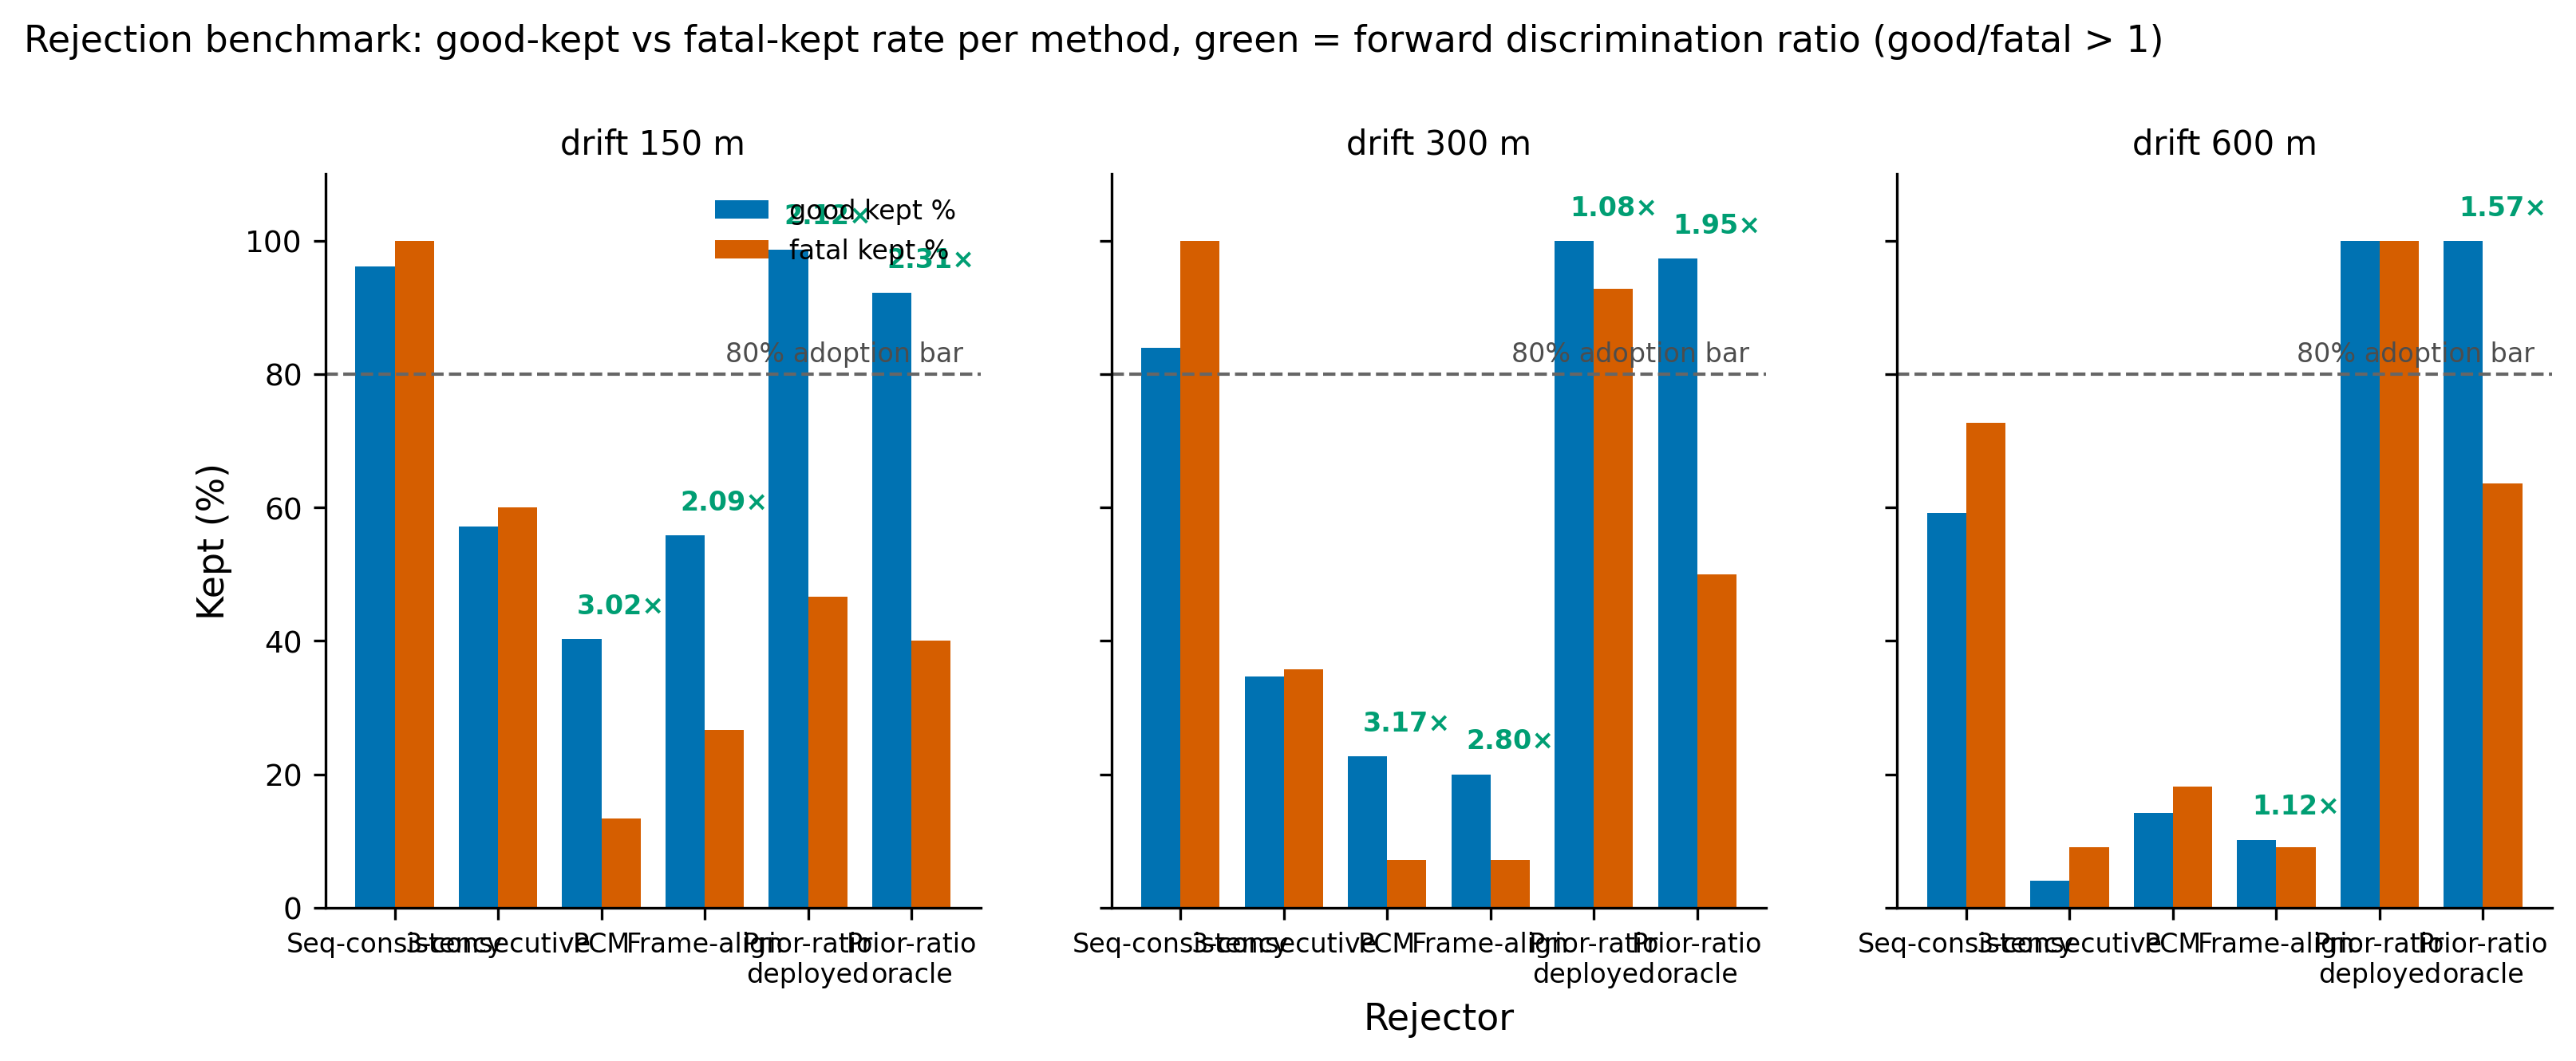
\includegraphics[width=\columnwidth]{figs/fig3_rejector_rates.png}
\caption{Backwards-rate benchmark over the pooled fix stream (255 accepted fixes). Bars: good-kept vs.\ fatal-kept percentage per rejector and drift; dashed line: the 80\% good-kept adoption bar. Sequential consistency and the three-keyframe rule keep fatals at $\geq$ good rates (ratio $\leq$1); PCM and frame alignment score $>$1 only by destroying coverage.}
\label{fig:rates}
\end{figure}

\subsection{Temporal coherence: the mechanism}
\label{sec:coherence}

\textbf{Setup.} Truth-referenced signed offsets, contiguous frames, R04 $n=610$ (alias $\geq$50\,m: 93; mid 20--50\,m: 374; good $<$20\,m: 143), R03 control $n=557$. Per-lag pair counts inline.

\begin{table}[t]
\caption{Median pairwise offset difference vs.\ frame lag (m). Null: offsets shuffled within group (10 trials). $n$ = alias pairs.}
\label{tab:coherence}
\centering
\begin{tabular}{@{}lcccc@{}}
\toprule
lag & $n$ & alias: med / null & good: med / null \\
\midrule
1 & 25 & 27.5 / 70.1 & \textbf{2.55$\times$ below null} \\
2 & 17 & 46.8 / 86.1 & 1.84$\times$ \\
3 & 15 & 27.9 / 63.9 & 2.29$\times$ \\
5 & 12 & 80.0 / 90.1 & 1.13$\times$ \\
8 & 11 & 60.3 / 93.5 & 1.55$\times$ \\
\bottomrule
\end{tabular}
\end{table}

\textbf{Finding 4---the alias offset is locally coherent and decays with lag.} Adjacent alias frames differ by 27.5\,m where random pairing gives 70.1\,m; the advantage decays to $\sim$1.1$\times$ by lag 5--8 (Fig.~\ref{fig:coherence}). The lock is not rigid: it drifts slowly (the period index changes occasionally), coherent over 2--4 frames. Correct fixes are independent per frame (at null at every lag, 0.78--1.13$\times$) and the R03 control matches them. The 20--50\,m band is \emph{partially} coherent---a mixture of alias and noise---which explains why threshold rejectors tuned anywhere in that band fail (Finding 1).

\begin{figure}[t]
\centering

\includegraphics[width=\columnwidth]{figs/fig2_coherence_curve.png}
\caption{Temporal coherence of the alias offset (R04, $n=610$ contiguous). Solid: median pairwise offset difference within the alias ($\geq$50\,m) and good ($<$20\,m) groups; dashed: shuffled nulls. The alias group sits 2.55$\times$ below its null at lag 1 and decays to $\sim$1.1$\times$ by lag 5--8; correct fixes are independent at every lag.}
\label{fig:coherence}
\end{figure}

\textbf{Consequence.} Within the coherence window, an alias chain is exactly as motion-consistent as the truth: pairwise consistency has a gauge symmetry (constant offsets cancel in frame differences), so PCM/sequential consistency are provably blind, not merely weak. Beyond the window, the offset has drifted enough to survive any tolerance that keeps good fixes (their own $\sim$17\,m scatter). The backwards rates of Sec.~\ref{sec:bench} are the statistical image of this geometry.

\subsection{The countermeasure fails for a measured reason}
\label{sec:counter}

\textbf{Setup.} Two routes: (a)~estimate the alias lattice from the map itself---detrended autocorrelation of a 500-px crop around each locked position, strongest local maximum in the 9.5--95\,m band, $n=610$; (b)~a multi-hypothesis mixture filter: candidate true positions on a $k\in[-4,4]$ lattice (period 20\,m, axis 171$^{\circ}$, from Sec.~\ref{sec:structure}), posterior from the prior likelihood, output $=$ posterior mean; prior uncertainty swept 5--300\,m in random-walk and IID forms. Kill criterion pre-registered: posterior-mean output must recover $\geq$30\% of the oracle gap (17.1\,m $\Rightarrow$ $\geq$5.1\,m) at prior $\sigma\leq$20\,m.

\textbf{Result (a)---the lattice is not in the map.} In-band periodicity is found on 9--17\% of frames (lowest for the alias group) and never aligns with the alias offset direction (median angular error 44--52$^{\circ}$, uniform). At 1.19\,m/px the satellite texture does not expose the furrow lattice the matcher locks onto.

\textbf{Result (b)---the mixture recovers nothing; MAP is actively harmful.} Baseline $k=0$ median 31.1\,m ($n=610$); single-axis oracle 14.0\,m (gap 17.1\,m). Posterior-mean output moves $-6.1\ldots+0.1$\,m across all prior forms and qualities (worst at $\sigma=50$ IID: $-6.1$\,m, far below the $\geq$5.1\,m bar); MAP output degrades to 68.4\,m at $\sigma=300$\,m. The failure is mechanical: frame differences cannot see a constant offset (Sec.~\ref{sec:coherence}), the prior is the only anchor, and the true offsets are not multiples of any single global lattice---the per-field revision of Sec.~\ref{sec:structure} at stream scale.

\textbf{Finding 5---recovery requires the per-field lattice, which no deployed signal provides.} The failure chain is closed: the alias offset is quantized along a field axis (Sec.~\ref{sec:structure}), the axis is not in the satellite texture (a), frame differences cannot see a constant offset (Sec.~\ref{sec:coherence}), and no prior tightness restores the modes (b). The 14.0\,m oracle is the non-degenerate bound for any matcher-side fix; the IID $\sigma=5$ mixture---the video-rate odometry limit---extracts nothing from it (31.2\,m).

\subsection{Held-out controls and the terrain boundary of the class}
\label{sec:heldout}

\begin{table}[t]
\caption{Terrain boundary of the alias class. Production match: drifted-prior solve rate, $n=40$ at d300. GT-tile solve: contiguous frames against the region's own satellite tile.}
\label{tab:terrain}
\centering
\begin{tabular}{@{}llcc@{}}
\toprule
Region & Terrain & Prod.\ match (d300) & GT-tile solve \\
\midrule
R03 & farmland & 34/40, 0 fatal & 557, good at null \\
R04 & furrow farmland & alias source & 610, alias class \\
R05 & mountain plateau & 1/40 & 5/100 (5\% ceiling) \\
R11 & desert & 34/40, 1 fatal & 199: 8 alias (4\%) \\
R02 & farmland/river & --- & 1/40 usable \\
R10 & orchard hills & --- & 0/40 usable \\
\bottomrule
\end{tabular}
\end{table}

The sub-tile coherent-alias class appears only on repetitive furrow farmland (R04). Desert and clean farmland are control terrain; the mountain plateau and the two additional held-out regions (R02, R10) belong to the \emph{unsolvable class} (a 0--5\% inlier ceiling even against the region's own ground-truth tile), which is a different, no-fix failure mode rather than a wrong-fix one.

\subsection{External replication: attempted and executed}
\label{sec:replication}

\textbf{Attempted replication 1---TEMPO-VINE (rejected on structure).} The most promising published agricultural dataset for this mechanism, TEMPO-VINE~\cite{tempovine}, provides RTK-grade GPS truth (1--2\,cm) in trellis and pergola vineyards---but its imagery is a forward-oblique RealSense D435 RGB-D camera on a ground rover at $\sim$1\,m height. Nadir aerial imagery matchable against satellite ortho does not exist in the dataset, so protocol requirement~1 fails and no measurement is possible. This is a \emph{structural} absence in the field: no public dataset currently pairs repetitive-crop aerial imagery with satellite references and continuous GPS.

\textbf{Executed replication 2---AerialVL (class absent; protocol guard fired).} We ported the full protocol to AerialVL, an independently collected UAV dataset (HuggingFace \texttt{hmf21/AerialVL}, cc-by-4.0, no paper; per-frame GPS in the image filenames; Qingdao, China; urban/coastal terrain)~\cite{aerialvl}. Two flight sequences were ingested (1{,}423 frames), the reference map built from the dataset's georeferenced ortho (0.959\,m/px), and protocol Steps 1--3 run.

\begin{table}[t]
\caption{AerialVL replication (protocol Steps 1--3).}
\label{tab:aerialvl}
\centering
\begin{tabular}{@{}lcc@{}}
\toprule
Metric & Seq 03-11 & Seq 03-16 \\
\midrule
Solved frames ($\geq$15 inliers) & 94/200 (47\%) & 0/200 (0\%) \\
Hole at zero & 5.3\% & --- \\
Axial resultant $R(180^{\circ})$ & 0.70 & --- \\
Anisotropy (along/perp) & 9.7$\times$ (16.3/1.7\,m) & --- \\
Median error & 17.1\,m & --- \\
Median offset vector & ($-$16.0 N, +4.1 E) 16.5\,m & --- \\
Good-group lag-1 coherence & \textbf{0.59$\times$ of null} & --- \\
Error groups (good/mid/alias) & 75 / 15 / 4 & --- \\
\bottomrule
\end{tabular}
\end{table}

Two findings follow. First, the alias class is \textbf{absent}: the alias tail is 4 frames (4.3\%), too thin for any coherence measurement. The sign-folding signatures that \emph{would} replicate (hole 5.3\%, $R$ 0.70, anisotropy 9.7$\times$) are produced by a different mechanism---a constant 16.5\,m common-mode georeferencing offset between the dataset's ortho and its drone GPS (spread 3.1\,m; a cross-validated bias correction removes 14\,m: 17.3$\to$3.3\,m). A constant offset is trivially ``perfectly coherent'', so this is a false-positive source for the diagnostic---and a live corroboration of Sec.~\ref{sec:coherence}'s gauge symmetry: a constant offset is invisible to any consistency-based rejection. Second, the protocol's own control guard fired: the \emph{good} group is temporally coherent (0.59$\times$ of its null; a clean dataset requires 0.8--1.25$\times$), meaning this dataset's GPS truth is temporally correlated---a benchmark-hygiene property worth reporting on its own, and a reminder that coherence checks must control for truth-correlation before interpreting alias coherence.

\textbf{Follow-up.} The one dataset class that could replicate the mechanism---repetitive-crop aerial imagery (the recently released ViLD dataset of UAV-to-satellite image matching over French fields, WACV 2026, access-gated~\cite{vild})---is stated as future work with the pre-registered protocol.

\section{Discussion}

\textbf{What the field should take.} (i)~Pooled A@$X$\,m metrics on repetitive terrain hide a failure class with full geometric support; signed-offset reporting is a cheap diagnostic that exposes it. (ii)~Robust-estimation defaults (PCM/GNC/sequential consistency) do not transfer to cross-view geo-localization on repetitive terrain: they fail backwards or at coverage-destroying purity, at measured rates. (iii)~The fix that works for one alias class (prior-ratio for whole-tile) does not exist for the other; hedging (posterior-mean) is safe but inert, mode-commitment (MAP) is dangerous (68.4\,m at $\sigma=300$). (iv)~An independent replication attempt shows the diagnostic's false-positive mode (constant georeferencing bias) and a truth-correlation guard that any future replication must pass.

\textbf{Limitations.} Dataset GPS truth ($\sim$10\,m class) bounds all absolute numbers---the R03 floor of $\sim$13\,m is plausibly the dataset's own noise floor, not the matcher. Sample sizes: per-region fatal counts are 5--14 per drift; all denominators are reported inline, and the key measurements ($n=32$ unanimity, $n=610$ coherence) do not rest on small cells. The sub-tile class is measured on a single region (R04) and does not replicate on clean or unsolvable terrain; an external dataset with repetitive-crop aerial imagery does not exist publicly. All rates are measured with one matcher (ORB+AKAZE+SIFT+MAGSAC); the coherence mechanism (Sec.~\ref{sec:coherence}) is matcher-independent, but rate magnitudes are matcher-conditional. AerialVL's georeferencing bias and correlated truth were discovered, not controlled for, in that replication.

\section{Conclusion}

We characterized a failure class in UAV-to-satellite geo-localization that consistency-based robustness tools cannot see: coherent-offset aliases, split into whole-tile (separable by a prior-ratio gate) and sub-tile (unreachable by any measured signal) classes. The sub-tile class defeats sequential consistency and the three-keyframe rule \emph{backwards} at measured rates, defeats PCM and frame alignment through coverage destruction, hides in magnitude histograms, and resists even the mechanism-motivated multi-hypothesis countermeasure, with a non-degenerate oracle bound of 14.0\,m median on the worst region against a 31.1\,m production baseline ($n=610$). The class is terrain-specific: absent on desert, clean farmland, mountain plateau, unsolvable regions, and an independent urban dataset. The paper contributes the taxonomy, the rate tables, the sign-folding diagnostic, and the quantified boundary of what map matching can and cannot recover---and, by exclusion, directs future work to per-field map annotation or odometry-quality regimes we quantify as unreachable at 7\,s frame spacing.

\section*{Data and Code Availability}
The measurement harness, rejector benchmark, coherence analysis, and replication scripts, together with all per-frame result artifacts backing every table and figure, are available from the authors; the replication protocol is fully specified (five steps, exact commands, pre-registered kill criteria) so that all experiments can be re-executed end to end. UAV-VisLoc is public~\cite{uavvisloc}; the AerialVL sequences used are public under cc-by-4.0~\cite{aerialvl}.

\bibliographystyle{IEEEtran}
\bibliography{refs}

\end{document}
